\documentclass[12pt,a4paper]{report}

% Balíčky
\usepackage[czech]{babel}
\usepackage[utf8]{inputenc}
\usepackage[T1]{fontenc}
\usepackage{hyperref} % klikací odkazy v PDF
\usepackage{graphicx} % vkládání obrázků
\usepackage{listings} % zvýrazňování kódu
\usepackage{xcolor} % nutné pro \definecolor
\usepackage{amsmath, amssymb}
\usepackage{titlesec} % balíček na formátování nadpisů

% Nastavení nadpisů
\titleformat{\chapter}[hang]
  {\normalfont\huge\bfseries}
  {\thechapter} % jen číslo kapitoly
  {1em}
  {}

% Nastavení pro zdrojové kódy
\definecolor{codebg}{RGB}{245,245,245}
\definecolor{codeframe}{RGB}{200,200,200}
\definecolor{keyword}{RGB}{0,0,180}
\definecolor{comment}{RGB}{0,128,0}
\definecolor{string}{RGB}{163,21,21}
\lstset{
    backgroundcolor=\color{codebg},
    frame=single,
    rulecolor=\color{codeframe},
    basicstyle=\ttfamily\small,
    keywordstyle=\color{keyword}\bfseries,
    commentstyle=\color{comment}\itshape,
    stringstyle=\color{string},
    numberstyle=\tiny\color{gray},
    numbers=left,
    stepnumber=1,
    numbersep=10pt,
    showstringspaces=false,
    breaklines=true,
    tabsize=4,
    captionpos=b
}

% ---- Začátek dokumentu ----
\begin{document}

% Úvodní stránka
\begin{titlepage}
    \centering
    {\Huge \textbf{Simulace paprskové optiky s grafickým rozhraním}\par} % No-Breaking Space
    \vspace{2cm}
    {\Large Dokumentace k maturitní práci\par}
    \vfill

    
\includegraphics[width=0.4\textwidth]{logo_gp.png}
    \vfill
    
    {\large Daniel Matouš\par}
    {\large Gymnázium, Praha 4, Písnická 760\par}
    {\large \today} % Uprav datum
\end{titlepage}

\pagenumbering{gobble}
% Abstrakt
\begin{abstract}
\paragraph{} Tato dokumentace popisuje grafické rozhraní pro program na simulaci paprskové optiky ve 2D prostoru. Cílem bylo vytvořit desktopovou aplikaci, jejíž GUI má všechny náležitosti očekávané od moderního rozhraní. Stanovil jsem si za cíl nepoužít jiné knihovny než ty, které jsou součástí základního Pythonu 3.14; všechny systémy projektu jsem se chtěl naučit vymyslet a implementovat sám.
\paragraph{} Pro projekt jsem vytvořil základ optické simulace, která v aktuálním stavu podporuje bodové zdroje libovolného počtu paprsků, odrážení od zrcadel a překážky, jež blokují paprsky. Podporuje přidávání dalších prvků odvozením od obecných tříd.
\paragraph{} Zásadním bodem cíle byl vlastní systém vybírání a přesouvání simulačních prvků pomocí myši metodou "Drag 'n drop".
\paragraph{} GUI bylo opatřeno i méně obvyklými prvky a ve svém aktuálním stavu vyladěno, ale není dost vybavené funkcemi, aby dovolilo uživateli využít všech možností simulace. Simulace sice poskytuje funkční základ, na kterém se dá expandovat, ale postrádá schopnosti, které jsem chtěl přidat.
\paragraph{} V průběhu tvorby jsem totiž zjistil, že bude komplikované zprovoznit i jen úplný základ. To se mi nakonec povedlo a v této dokumentaci vás provedu jeho tvorbou, fungováním a dalším využitím.
\end{abstract}

% Obsah
\setcounter{tocdepth}{2} % Uprav úroveň nadpisů v obsahu
\tableofcontents
\newpage
\pagenumbering{arabic}

% Úvod
\chapter{Úvod}
\paragraph{} Jakmile jsem zjistil, že předmětem závěrečného ročníku bude tvorba maturitního projektu, věděl jsem, že chci tvořit grafické rozhraní. Tím jsem si byl od začátku jistý nejen proto, že to je oblast, která mě zajímá a chci se v ní zlepšovat, ale také proto, že v budoucnu bych chtěl pracovat právě na vývoji nástrojů s GUI. Dále mi bylo jasné, že budu chtít tvořit čistě softwarový projekt bez hardwarové součásti, protože s prací s hardwarem nemám žádné dobré zkušenosti.
\paragraph{} Výběr platformy pro mě byl také jasný. Mám zkušenosti s Pythonem a jeho knihovnou Tkinter, které bych si rád prohloubil.
\paragraph{} Jako obsah své práce jsem si vymyslel vykreslování paprskové optiky, protože to je záležitost, která se bez dobrého grafického rozhraní neobejde, a proto jsem počítal s tím, že nechá práci na GUI vyniknout. Při sepisování požadavků pro svou simulaci jsem počítal s využitím jako program, který by studenti mohli využít při studiu optiky pro prohloubení intuice nebo profesoři pro vytváření obrázků optických soustav bez nutnosti používat online nástroje nebo placené nástroje. V plánu jsem tedy měl plno simulačních prvků, které by zajistily, že pomocí nich bude možno vytvořit téměř cokoliv, co by uživatel mohl chtít.
% \paragraph{} Udělat tak všestranný program, aby se stal pro někoho první volbou pro práci s optikou, se mi upřímně nepovedlo. % Vykomentováno z úvodu - není součást zhodnocení na začátku
\paragraph{} Existují již nástroje, které dělají vše, co můj, a ještě mnohem víc. Na jeden takový nástroj, \href{https://phydemo.app/ray-optics/simulator/}{PhyDemo Ray Optics Simulator}, mě upozornil můj profesor ihned poté, co jsem tento nápad na projekt navrhl. Mým cílem zde ale není vyvinout program schopný konkurovat ve schopnostech projektům od mnohem zkušenějších vývojářů (nebo týmů vývojářů), než jsem já, nýbrž ukázat na funkčním příkladu, co umím vytvořit pomocí své oblíbené GUI knihovny.
\newpage
\paragraph{} Cílem tohoto tématu bylo naučit se co nejvíc o tvorbě uživatelského rozhraní a konkrétně o tvorbě pomocí Tkinteru. Kromě využití základních schopností je součástí projektu také použití pokročilejších funkcí knihovny, použití událostmi řízeného programování a využití rozšiřujícího modulu \lstinline{Tkinter.ttk}.
\paragraph{} V této dokumentaci najdete informace k fungování projektu a k tomu, jak jej používat. Nejdříve naleznete programátorskou dokumentaci, pak následuje uživatelská dokumentace. V programátorské části je vysvětlena struktura mého projektu a jsou tam popsány nejdůležitější součásti projektu. Popsáno je nejprve i prostředí, ve kterém jsem pracoval a rovněž použité knihovny. Uživatelská dokumentace se sestává z návodu na instalaci a spuštění programu a z návodu k použití.

% Programátorská dokumentace
\chapter{Programátorská dokumentace}
\paragraph{} V programátorské dokumentaci vás seznámím nejdříve s použitými vývojovými nástroji, pak se základními principy, na kterých můj projekt funguje a potom vše rozeberu více do hloubky v částech postupně o stavbě grafického rozhraní, souborové struktuře, matematické simulaci a nakonec popíšu, jak se v kódu projektu orientovat a přiblížím vše potřebné pro ty, kdo by v něm chtěli dělat změny. Relevantní příklady kódu, na kterých zamýšlím něco ukázat, budou doprovázet celou tuto kapitolu.
\section{Použité technologie a nástroje}
\begin{itemize}
    \item Programovací jazyk: Python. S Pythonem mám předchozí zkušenosti a hodí se pro tento typ projektu proto, že poskytuje dobré možnosti pro práci s OOP a je připravený na využití knihovny Tkinter, kterou chci používat.
    \item Knihovny:
    \begin{itemize}
        \item \lstinline{Tkinter}: Defaultní knihovna Pythonu, název je zkratka z "Tk Interface".
    Knihovna Tkinter byla vytvořena v roce 1991 a rozhraní v ní vytvořená vypadají dnes krajně zastarale. Mě se tento vzhled líbí, proto toto nepovažuji za negativum a pokusil jsem se tohoto stylu držet. V Tkinteru lze tvořit i moderně vypadající okna, a to obzvlášť díky modulu "\lstinline{ttk}", který dovoluje tvorbu vlastních stylů.
    \item Modul \lstinline{Tkinter.ttk}: Modul, který je součástí knihovny Tkinter. Je to zkratka z "Themed Tk" a dovoluje používat několik nových grafických prvků a definovat a používat vlastní styly. Já z \lstinline{Tkinter.ttk} používám prvky \lstinline{PanedWindow, Separator, LabelFrame, Notebook} a \lstinline{Sizegrip}, které mnou vytvořenému grafickému rozhraní dávají dnes již časté moderní vymoženosti.
    \item Modul \lstinline{Tkinter.filedialog}: Modul, který je součástí Tkinteru a poskytuje předpřipravené funkce pro vyvolání okna na výběr souborů pro načtení nebo uložení. Vzhled oken je uzpůsoben tak, jak je uživatel zvyklý ze všech ostatních programů, které dovolují otevírání a tvorbu souborů a jejich vzhled se přizpůsobuje vzhledu operačního systému.
    \item \lstinline{Math}: Standardní knihovna Pythonu, která do mého programu dodává matematické funkce potřebné při výpočtech v analytické geometrii. Z \lstinline{Math} používám funkce \lstinline{radians, sin, cos, sqrt,} \newline\lstinline{atan2, degrees}.
    \item \lstinline{Random}: Standardní knihovna Pythonu, kterou využívám pouze pro generaci náhodných čísel do jmen objektů pro jejich odlišení.
    \item \lstinline{Json}: Knihovna, která zprostředkovává konverzi Python objektů do textové reprezentace ve formátu \lstinline{Json} a také konverzi zpět z \lstinline{Json} formátu na Python objekty. Používám tyto funkce pro uložení dat do souboru a načtení dat ze souboru.
\end{itemize}
\item IDE: Visual Studio Code s rozšířením pro Python. Již s ním mám zkušenosti a přes přechodné problémy se zprovozněním Python debuggeru, které jsem vyřešil během začátku projektu, funguje bezproblémově.
\item Verzovací systém: Git se vzdáleným repozitářem uloženým na Githubu. Jakožto budoucí student informatiky potřebuji být schopen Git hladce používat. Tento projekt mi poskytl výbornou možnost se s Gitem, se kterým jsem neměl předchozí zkušenosti, naučit pracovat.
\item Dokumentace: Vytvořena v \LaTeX u za pomocí stránek Overleaf. Používám knihovny \lstinline{Graphics, Listings} a \lstinline{Xcolor} a další.
\end{itemize} Během žádné části projektu nebyla využita AI.
\newline
\section{Využívané programovací koncepty}
\paragraph{} Všechny části projektu ve vysoké míře využívají OOP. Většina souborů projektu poskytuje třídy, se kterými pak \lstinline{main.py} pracuje. Vstup je zajišťován za pomoci Tkinteru prostřednictvím funkcí \lstinline{Widget.bind()} a vestavěného systému událostí (eventů). Využito je tedy událostmi řízené programování, zatímco hlavní proces je po inicializaci GUI ponechán v nekonečném cyklu \lstinline{Tk.mainloop()}.
\paragraph{} Kromě událostí (jako třeba eventů myši \lstinline{<Motion>, <1> a <B1-Motion>} a virtuálních eventů \lstinline{<<ComboboxSelected>> a <<NotebookTabChanged>>}) používám metodu \lstinline{trace} náležící Tkinter třídám \lstinline{StringVar a IntVar} (a \lstinline{DoubleVar a BooleanVar}, tyto ale nepoužívám), která dovoluje nastavit "callback funkci", která má být zavolána v momentě, kdy je do té proměnné vepsána nová hodnota. To se mi velmi hodilo u dynamicky generovaného \lstinline{Spinbox} widgetu v editovacích panelech - má totiž tři způsoby, jak v něm hodnota může být změněna, a přiřazení funkce pomocí \lstinline{StringVar.trace} si se všemi třemi možnostmi elegantně poradí univerzálním způsobem.
\begin{lstlisting}[language=Python, caption=Přiřazení metody edit\_size pomocí Tkinter trace]
    # Width entry field
    self.var_width = tk.StringVar()
    self.var_width.set(self.x1 - self.x0) # Set to current width
    self.var_width.trace("w", self.edit_size) # Takes care of all three types of setting
    
    self.spb_width = tk.Spinbox(master=frm, textvariable=self.var_width, from_=1, to=100000)
    self.spb_width.grid(row=1, column=1)
\end{lstlisting}
\section{Drag 'n drop}
\paragraph{} Zásadním bodem cíle byl vlastní systém vybírání a přesouvání simulačních prvků pomocí myši metodou "Drag 'n drop", což dovoluje rychle i přesně přemisťovat prvky a je nepostradatelnou součástí každého moderního GUI ovládajícího program, jako je můj.
\paragraph{} Drag 'n drop je vytvořen za pomoci systému událostí přítomném v Tkinteru. Když uživatel stiskne tlačítko, je zavolána funkce \lstinline{get_mouse_selected},\newline která dostane jako argument událost, ze které získá souřadnice, na kterých událost vznikla, tedy souřadnice kliknutí. Zeptá se \lstinline{Tkinter Canvas} widgetu, jaké objekty se na tomto místě nacházejí. Jako odpověď dostane interní ID objektů na canvasu. Pro každé toto ID se poté zeptá canvasu pomocí funkce \lstinline{Canvas.type(id)}, jaký je typ toho objektu. Všechny objekty, které jsou čáry, jsou ignorovány. Tímto získá seznam překážek, které uživatel právě chytil. Uloží je do seznamu. Pokud je aktuální režim vybírání "Vrchní překážka", vybere a uloží jen tu nejvíc vrchní z překážek, co najde pod kurzorem.
\paragraph{} Zároveň vyvolá dynamické vygenerování editovacího panelu.
\paragraph{} Pohnutí myší s podrženým levým tlačítkem vyvolá spuštění funkce \newline \lstinline{mouse_drag}, která tento seznam používá. Na všech těchto objektech zavolá jejich \lstinline{move(x, y)} metodu o příslušný počet pixelů. Aktualizuje také souřadnice zobrazené v editovacím panelu.
\newline
%\newpage % So the listing is on a new page
\begin{lstlisting}[language=Python, caption=Začátek funkce get\_mouse\_selected]
def get_mouse_selected(event: Event, screen: Screen) -> list[int]:
    # Set variables based on selection mode
    selection_mode = constants.selection_mode
    if constants.debug_selection:
        print(f"Mode: {selection_mode}")
    match selection_mode:
        case "SINGLE":
            offset = constants.single_select_offset
        case "MULTI":
            offset = constants.multi_select_offset
        case "LINES":
            offset = constants.lines_select_offset
        case _:
            raise Exception("Selection mode does not match expected cases")
        
    x0 = event.x - offset
    x1 = event.x + offset
    y0 = event.y - offset
    y1 = event.y + offset
    overlapping = screen.tk_canvas.find_overlapping(x0, y0, x1, y1) # From the documentation for tk.Canvas.find_overlapping(): "The items are returned in stacking order, with the lowest item first" 

    if len(overlapping) == 0: # If nothing selected, nothing selected
        return []
\end{lstlisting}
\section{GUI}
\paragraph{} Uživatelské rozhraní je rozděleno na tři panely. Levý panel je ponechaný prázdný, zde můžou být v budoucnu přidány dodatečné ovládací prvky, nebo doimplementován widget \lstinline{Treeview}, který tento panel zatím vyplňuje a mohl by v budoucnu podávat přehled o hierarchii objektů na jednotlivých plochách. Funkce GUI jsou blíže popsány v uživatelské dokumentaci, zde se zaměřím na použité widgety.
\paragraph{} Kopírovat sem kód incializující GUI by byla škoda místa, proto raději uvádím výčet použitých widgetů:
\begin{itemize}
    \item Z Tkinteru: \newline\lstinline{Menu, Toplevel, Label, Frame, Labelframe, Button, Entry,}\newline\lstinline{Canvas, Spinbox}
    \item Z Tkinter.ttk: \begin{itemize}
        \item \lstinline{Notebook}: Na přepínání mezi plochami systémem karet
        \item \lstinline{Panedwindow}: Rozdělení hlavní části okna na tři panely, jejichž hranice se dají vůči sobě posouvat
        \item \lstinline{Separator}: Dekorační detail - dělicí čáry v liště nástrojů a editovacím panelu
        \item \lstinline{Sizegrip}: Úchyty na chycení okna pro resizování. Hodně se mi líbí jejich vzhled, proto jsem použil rovnou dva
        \item \lstinline{Combobox}: Nastavování několika věcí: Režim drag 'n drop výběru, typ a tvar přidávaného objektu, výběr plochy k odstranění
    \end{itemize}
\end{itemize}
\paragraph{} Během tvorby GUI jsem dbal na resizovatelnost okna (použitím několika Frame widgetů a konfigurováním \lstinline{weight} parametrů pro řádky a sloupce v grid manageru) a to jsem zohlednil i použitím widgetů \lstinline{Panedwindow} a \lstinline{Sizegrip}.
\paragraph{} Chtěl jsem si vyzkoušet design vícero způsobů, jak něco konfigurovat, proto několik věcí používá \lstinline{ttk.Combobox}, číselné vstupy pro šířku a výšku používají \lstinline{Spinbox}, menu přidávání a odstraňování ploch používají \lstinline{Toplevel} okna a textové vstupy u přidávání ploch používají prvek \lstinline{Entry}. Líbí se mi, že i přes moje malé množství předchozích zkušeností mi dovolil Tkinter zahrnout do projektu tak pestrý výběr rozhraní.
\paragraph{} Jsem rád, že jsem si vyzkoušel i dynamické generování widgetů do editovacího panelu, protože to je něco, co jsem si už delší dobu chtěl vyzkoušet. Dekorační prvek \lstinline{Labelframe}, který jsem použil na ohraničení editovacího panelu, se mi vzhledově líbí a těšil jsem se, až se mi naskytne šance jej v nějakém projektu využít.
% Sem jsem přesunul zhodnocení z úvodu
\paragraph{} Jak bylo již zmíněno, součástí mého tématu a plánu jeho realizace bylo využití pokročilejších schopností knihovny \lstinline{Tkinter}, včetně používání značek (tagů) pro identifikaci objektů na plochách a dále včetně událostmi řízeného programování a využití rozšiřujícího modulu \lstinline{Tkinter.ttk}.
\paragraph{} Naučil jsem se toho hodně jak o principech tvorby grafického rozhraní a mnoha často používaných konceptech (práce s mřížkou, resizování prvků, drag 'n drop, událostmi řízené programování), tak o Tkinteru samotném (tvorba menu lišty, systém událostí v Tkinteru, Canvas tagy). Dokážu nyní s touto knihovnou efektivně pracovat a chápu její součásti. Důvěrně jsem se seznámil i s widgety z jejího rozšiřujícího modulu \lstinline{Tkinter.ttk} ($\mathbf{ttk} = \bold{T}$hemed $\mathbf{Tk}$inter).
% TODO New page?
\section{Simulace}
\paragraph{} Vytvořil jsem systém pro ukládání a vykreslování segmentů paprsků na \lstinline{Tkinter Canvas}. Paprsek může být definován buď dvěma body, nebo jedním bodem a jedním úhlem, což se hodí pro segmenty, u kterých není znám koncový bod, protože ještě neprošly kolizí nebo mají jít až do nekonečna a tedy být vykresleny až k okraji plochy.
\paragraph{} Třídy podílející se na paprskové simulaci jsou \lstinline{Source, Segment} a obecná třída \lstinline{Interactor} a třídy od ní odvozené. Tyto třídy jsou všechny opatřeny typovými anotacemi jakožto i komentáři, proto je tato podkapitola neprobírá všechny do hloubky. Představím zde ale alespoň třídu \lstinline{Segment} a pak \lstinline{Source}.
\paragraph{} Součástí simulace je také systém pro vyřizování kolizí a postupnou generaci nových segmentů, jak jde paprsek dál a podstupuje kolize, při kterých se generují jeho nové segmenty.
\paragraph{} Níže jsou popsány dvě ze tříd tvořících kostru mého programu. Nacházejí se v \lstinline{core_classes.py} a pokud chcete měnit něco v jádru programu, bude se vám hodit tento přehled.
\begin{lstlisting}[language=Python, caption=třída Segment]
class Segment:
    def __init__(self, start_x: int, start_y: int, angle: float, end_specified: bool =False, end_x: int =None, end_y: int =None, visible: bool =True):
        self.start_x: int = start_x
        self.start_y: int = start_y
        self.angle: float = angle
        self._end_specified: bool = end_specified
        self._end_x: int | None = end_x
        self._end_y: int | None = end_y
        self.visible: bool = visible
        self.last_collided_interactor = None
        self.last_collided_line = None
    def __str__(self):
        return f"Segment with X: {self.start_x} Y: {self.start_y} Angle: {self.angle}"
    def specify_end(self, x, y) -> None:
        self._end_x = x
        self._end_y = y
        self._end_specified = True
\end{lstlisting}
\paragraph{} \lstinline{Segment} popisuje jeden segment paprsku. Je definován buď startovním bodem a úhlem, nebo startovním bodem a koncovým bodem. Moje renderovací funkce si poradí s oběma způsoby definování. Často je segment vytvořen s informací o počátečním bodu a úhlu a později mu je určen koncový bod. Pro tento přechod lze použít metodu \lstinline{Segment.specify_end(x, y)}, která správně nastaví proměnné. Je doporučeno používat tuto funkci, protože je kratší, než všechny tři proměnné nastavovat manuálně a také to zamezí případům, kde by člověk zapomněl nastavit atribut \lstinline{_end_specified}. Proto jsou atributy \lstinline{_end_x}, \lstinline{_end_y} a \lstinline{_end_specified} označeny jako soukromé atributy. Funkce \lstinline{__str__()} je dostupná pro pohodlnější debugování.
\newpage
\begin{lstlisting}[language=Python, caption=třída Source]
class Source:
    def __init__(self, x: int, y: int, angle: float) -> None:
        self.x: int = x
        self.y: int = y
        self.angle: float = angle
        self.generated_segments: list[Segment] = []
    def __str__(self) -> str:
        return f"Source with X: {self.x} Y: {self.y} Angle: {self.angle} Number of segments: {len(self.generated_segments)}"
    def generate_segments(self, parent_screen: Screen) -> None:
        ...
\end{lstlisting}
\paragraph{} Zdroj paprsku je definován jen svými souřadnicemi \lstinline{x} a \lstinline{y} a svým úhlem. Při spuštění funkce \lstinline{Source.generate_segments} vygeneruje zdroj první paprsek s právě těmito souřadnicemi a úhlem a další segmenty k paprsku přidává podle výsledků kolizí. Aby zdroj paprsku mohl získat data o kolizích, potřebuje dostat při zavolání této funkce odkaz na instanci plochy, na které se nacházejí prvky, se kterými bude interagovat. Z instance plochy získá seznam simulačních prvků, se kterými postupně se všemi nechá pomocí funkcí z modulu \lstinline{collisions.py} vypočítat kolize. Všechny kolize, které neuspěly, jsou odhozeny. Z kolizí úspěšných vybere tu nejbližší k začátku posledního svého segmentu, tedy tu, na kterou paprsek narazí jako první. Segmenty vygenerované touto kolizí přidá ke svému paprsku tím, že je přidá do svého seznamu \lstinline{generated_segments}. Opět je dostupná \lstinline{__str__()} funkce, která vrací sesumírované podrobnosti o instanci.
\paragraph{} Knihovna \lstinline{Math} poskytuje funkce nepostradatelné při geometrických výpočtech, vyskytujících se právě v simulační části, ale zároveň se stala zdrojem jednoho z nejvíce absurdních bugů mého projektu, rozebraného níže.
\newline %TODO
\begin{lstlisting}[language=Python, caption=Využití math.atan2() v geometrickém výpočtu]
    vector_line = (line_x2 - line_x1, line_y2 - line_y1)
    ...
    return_dict["line_angle"] = degrees( atan2(vector_line[1], vector_line[0]) )
\end{lstlisting}
\paragraph{} Funkce \lstinline{math.atan2(y, x)} mi způsobila asi týden trvající zádrhel, při kterém jsem přezkoumával každou část svých funkcí na geometrické výpočty, abych našel záludnou chybu. Požaduje totiž jako argumenty souřadnice vektoru a to v pořadí \lstinline{y, x}, čehož jsem si nevšiml ve spěchu, když jsem chtěl implementovat odrazy co nejdříve. Argumenty jsem podával v pořadí \lstinline{x, y} a moje kolize pak vracely úhly nesprávné, ale zároveň dostatečně smysluplné na to, aby člověk začal podezřívat svoje vzorce a svoje chápání analytické geometrie, nikoliv nenápadné dosazení do funkce.
\section{Debugovací funkce}
\paragraph{} Projekt obsahuje debugovací funkce, které mi pomáhaly při hledání chyb a potvrzování, že vše funguje tak, jak má, a určitě pomůžou i všem ostatním, kdo by se chtěl mým projektem blíže zabývat nebo do něj něco přidávat. Klasické debugovací nástroje jako VSCode s Python debuggerem samozřejmě stále jsou nejdůležitějším nástrojem.
\section{Známé chyby}
\paragraph{} Projekt není bezchybný. Když uživatel přepne na obrazovku, kterou předtím ještě neměl otevřenou - tedy jednu z předpřipravených obrazovek, kterou ještě neotevřel, nebo vlastní obrazovku načtenou ze souboru - tak mohou být paprsky vykresleny špatně, a to tím způsobem, že v místě změny směru jsou segmenty vykresleny špatným směrem. Původ chyby lze podle mě hledat v části zodpovědné za kolize nebo za renderování parpsku. Když se mi nepovedlo najít zdroj chyby, vyřešil jsem problém přidáním tlačítka na aktualizaci obrazovky. Zároveň se program pokusí přerenderovat paprsky při přepnutí mezi plochami a díky tomu se často chybné vykreslení spraví i tím, když přepnete na jakoukoliv jinou plochu a pak zpátky na tu s chybným zobrazením.
\paragraph{} V nějakých na první pohled naprosto náhodných případech selže výpočet kolizí s odrazy a paprsek se neodrazí. Problém patrně tkví ve funkcích na výpočty kolizí a odrazů, ale komplexita mého systému pro tyto výpočty mi nedovolila včas chybu opravit. Narazí-li uživatel na takovou chybu, stačí zrcadlem nebo zdrojem paprsku pohnout byť o jeden pixel.
\newpage % So the image ends up on the same page
\section{Architektura souborů projektu}
Hierarchie souborů kódu mého projektu je:
\begin{figure}[h]
    \centering
    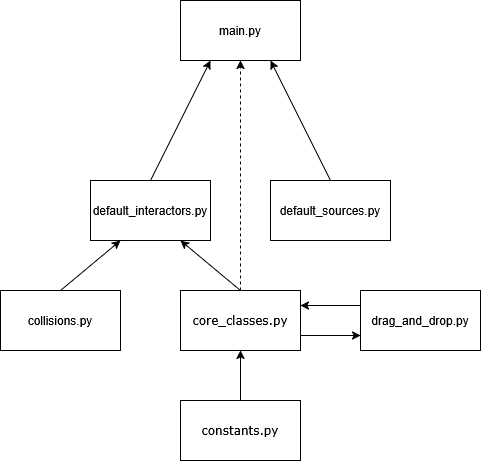
\includegraphics[width=0.5\linewidth]{Dependency_tree.png}
    \caption{Graf dependencí}
\end{figure}
\paragraph{} Šipka indikuje, odkud kam se importuje. Součásti položené nahoře v hierarchii závisí na těch pod nimi a postupně na nich staví. Popis jednotlivých částí:
\paragraph{} \lstinline{constants.py}: Soubor konstant využívaných ostatními částmi. Nahoře jsou konstanty měnitelné, kterými je možno přizpůsobit některé charakteristiky programu (vypnout načítání demonstračních ploch při spuštění, vypnout veškeré printování do konzole, změnit font dolní lišty, změnit barvu paprsků, změnit maximální povolený počet segmentů v paprsku, než sebekontrola programu automaticky ukončí paprsek\dots). Dole se nachází interně používané konstanty.
\paragraph{} \lstinline{core_classes.py}: Obsahuje hlavní třídy projektu - jeho základ.
\paragraph{} \lstinline{drag_and_drop.py}: Obsahuje kód pro výběr pomocí myši a přesun objektů. Stará se také o vyvolání updatů pravého panelu.
\paragraph{} \lstinline{default_interactors.py}: Definuje předem vytvořené simulační prvky.
\paragraph{} \lstinline{default_sources.py}: Definuje předem vytvořené generátory paprsků.
\paragraph{} \lstinline{main.py}: Je určen ke spuštění programu, obsahuje kód pro GUI a vytváří demonstrační plochy při otevření programu.
\section{Formátování kódu}
\paragraph{} Tato část se týká mých vlastních rozhodnutí o detailech toho, jak má být můj projekt formátován. Jsou to věci, o kterých píšu pro přiblížení toho, proč jsou některé věci napsané tak, jak jsou. Není to nic kriticky důležitého pro samotné fungování projektu, takže je to až zde jako poslední bod dokumentace pro programátory.
\paragraph{} Soukromé atributy jsou označeny podtržítkem na začátku, třeba \newline\lstinline{_end_specified} ve tříde \lstinline{Segment}. Python soukromé atributy neskrývá, proto můžete napsat kód, který je bude měnit přímo. To se ale nedoporučuje proto, že na práci s nimi jsou dostupné třídní metody, které jsou na jejich správné nastavení nebo přečtení přímo vytvořené.
\paragraph{} Co možno nejvíc argumentů funkcí, atributů tříd a jiných proměnných jsem vybavily typovými anotacemi pro jednodušší práci s nimi a rychlejší hledání chyb.
\begin{lstlisting}[language=Python, caption=Konstruktor třídy Source opatřený typovými anotacemi argumentů i atributů]
class Source:
    def __init__(self, x: int, y: int, angle: float, editing_name: str ="Zdroj", editing_type: str = "Zdroj paprsku") -> None:
        self.x: int = x
        self.y: int = y
        self.angle: float = angle
        self.generated_segments: list[Segment] = []

        # attributes specific to the editing panel
        self._editing_name: str = f"{editing_name} #{id(self)}"
        self.editing_type: str = editing_type
        self._editing_frame_generated: bool = False
        self._editing_frame: None | tk.Frame = None
\end{lstlisting}
\newpage % looks better
\paragraph{} Co se týče uspořádání kódu v souborech, úplně nahoře jsou importy z jiných souborů mého projektu, pod nimi je volný řádek a pod tím jsou importy standardních Python knihoven.
\begin{lstlisting}[language=Python, caption=Styl importů z core\_classes.py]
import constants

import tkinter as tk
from tkinter import ttk # Just for one type annotation and a Combobox
from tkinter.filedialog import askopenfile, asksaveasfile
from math import tan, radians
from json import dumps, loads
\end{lstlisting}
Názvy proměnných následují pravidla americké angličtiny, protože tu používají názvy v Pythonu a Tkinteru. Komentáře jsou napsané britskou angličtinou, protože tu používám já. Je to maličkost, kterou uvádím hlavně pro objasnění pro ty, kdo by se pozastavili nad tím, že používám jiný pravopis v názvu funkce a jiný v komentáři hned vedle. V kódu dbám na to, aby se pravopis shodoval s názvy proměnných v Tkinteru a v komentářích dbám na to, aby se shodovaly s mými poznámkami a mými shrnutími commitů v Git repozitáři.
\paragraph{Ohledně debugování}
\enlargethispage{2\baselineskip}
\paragraph{} Jelikož člověk, který chce můj kód debugovat, má můj kód jistě již otevřený v editoru, zapíná se debugování přímo přepsáním \lstinline{True/False} v kódu. V \lstinline{constants.py} se nachází sekce určená nastavení, zda jsou debugovací funkce aktivní. Kromě hlavního nastavení, kterým lze zapnout a vypnout veškeré debugovací vypisování, je funkčnost rozdělena na několik druhů podle toho, jaký systém mého projektu chce člověk zkoumat. Může je zapínat postupně, aby konzole nebyla spamována nekonečnými \lstinline{print} statementy, které si člověk nevyžádal. Nejpodstatnější nastavení:
\begin{itemize}
    \item \lstinline{debug_any}: Hlavní nastavení. Pokud je vypnuto, vypne všechno debugování kromě vypsání zprávy při vypnutí.
    \item \lstinline{debug_warnings}: Zapíná varování do konzole o věcech, které samy o sobě nejsou kritickou chybou, ale mohly by činit problémy jinde, jako třeba počítání s úhly mimo rozmezí \lstinline{0} až \lstinline{360}. Takovéto chyby se můj kód snaží nacházet a upozornit na ně. Všechna varování začínají \newline"\lstinline{WARN: }". Pokud něco nefunguje a jsou při tom vypisována varování, zdroj těchto varování je první místo, kam by se člověk měl podívat, protože tam asi vězí chyba.
\end{itemize}

% Uživatelská dokumentace
\chapter{Uživatelská dokumentace}
\section{Instalace a spuštění}
\paragraph{} Pro používání stačí stáhnout složku obsahující soubory programu a spustit soubor main.py. Ten importuje všechny potřebné součásti a spustí okno programu. Po zavření okna se zavře zbytek programu.
Projekt je závislý na aktuální verzi Pythonu, Python 3.14, a na knihovnách \lstinline{Math} a \lstinline{Tkinter}, obě jsou defaultní součástí Pythonu a jsou s každou jeho instalací defaultně předinstalované.
\paragraph{} Stačí tedy stáhnout Python 3.14 a program spustit. Otevře se okno aplikace a načtou se předpřipravené demo plochy, na kterých si může člověk prohlédnout a vyzkoušet, co program umí.
\begin{figure}
    \centering
    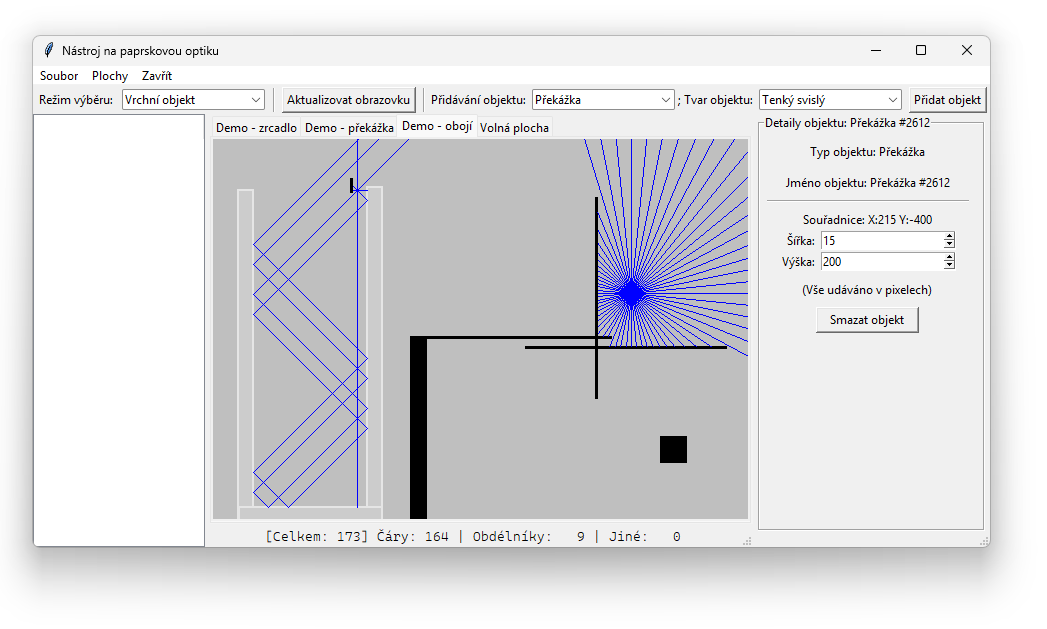
\includegraphics[width=1\linewidth]{Reference_GUI_small.png}
    \caption{Grafické rozhraní s uživatelem vytvořenou simulací a spočtenými objekty}
    \label{fig:placeholder}
\end{figure}
\newpage\section{Popis GUI}
\paragraph{} Uživatelské rozhraní je rozděleno na tři panely. Prostřední panel je největší a nachází se na něm hlavní pracovní plocha programu. Při škálování aplikace také dostává prioritně nový prostor, zůstává tedy největším. V horní části naleznete lištu s několika záložkami. Myší a pak i šipkami na klávesnici lze mezi záložkami přepínat a tím určovat, která plocha je aktuálně zobrazena na hlavní ploše programu. Nahlédněte pod hlavní plochu a najdete lištu, na kterou se při každé změně na obrazovce vypíšou aktuální údaje o tom, kolik je na dané ploše vykresleno čar, obdélníků a jiných útvarů. Celkový počet objektů je k přečtení nalevo. Použit je font typu monospace, aby se předešlo cukání při změně počtu cifer v číslech.
\enlargethispage{2\baselineskip}
\begin{samepage}
\paragraph{} Panel napravo slouží k zobrazení detailů o vybrané položce. Pokaždé, když kliknete na nějaký objekt nebo jím myší přetáhnete, je vybrán a zobrazí se zde jeho typ a jeho název. Výběr zrušíte kliknutím na volné pozadí pracovní plochy. Jména objektů obsahují náhodná čísla pro odlišení od sebe. Zároveň se zde pod oddělovací čarou objeví při vybrání zrcadla nebo překážky editovací panel, ve kterém lze sledovat aktuální souřadnice objektu a také měnit výšku a šířku, což se ihned promítne na simulační ploše. Dole v editovacím panelu je tlačítko pro smazání objektu.
\end{samepage}
\paragraph{} V horní části okna, nad hlavní částí, se nachází nástrojová lišta a nad ní tenká lišta s menu. Nástrojová lišta se sestává ze tří částí oddělených vertikálními čarami. V první lze nastavit režim vybírání myší pro systém drag 'n drop. V druhé se nachází tlačítko na aktualizování simulace a překreslení na obrazovku. Ve třetí části můžete ve výběru vybrat jeden z vícero druhů objektů, co přidat. Dostupné jsou zrcadlo, překážka a světelné zdroje o různém počtu paprsků. V druhém výběru v této části lze nastavit, jaký tvar bude mít přidané zrcadlo nebo překážka. Tlačítko hned vedle přidá na obrazovku objekt s požadovanými vlastnostmi. Pokud přidáváte světelný zdroj, pole "Tvar objektu"{} nemá žádný efekt. Tvar u zrcadel a překážek lze měnit podrobněji později pomocí editoru v pravé části aplikace.
\paragraph{} Nad panely se nachází lišta menu se třemi tlačítky, sem lze v budoucnu přidávat další tlačítka. Jejich funkce jsou blíže vysvětleny v sekci níže.

\begin{figure}[h]
    \centering
    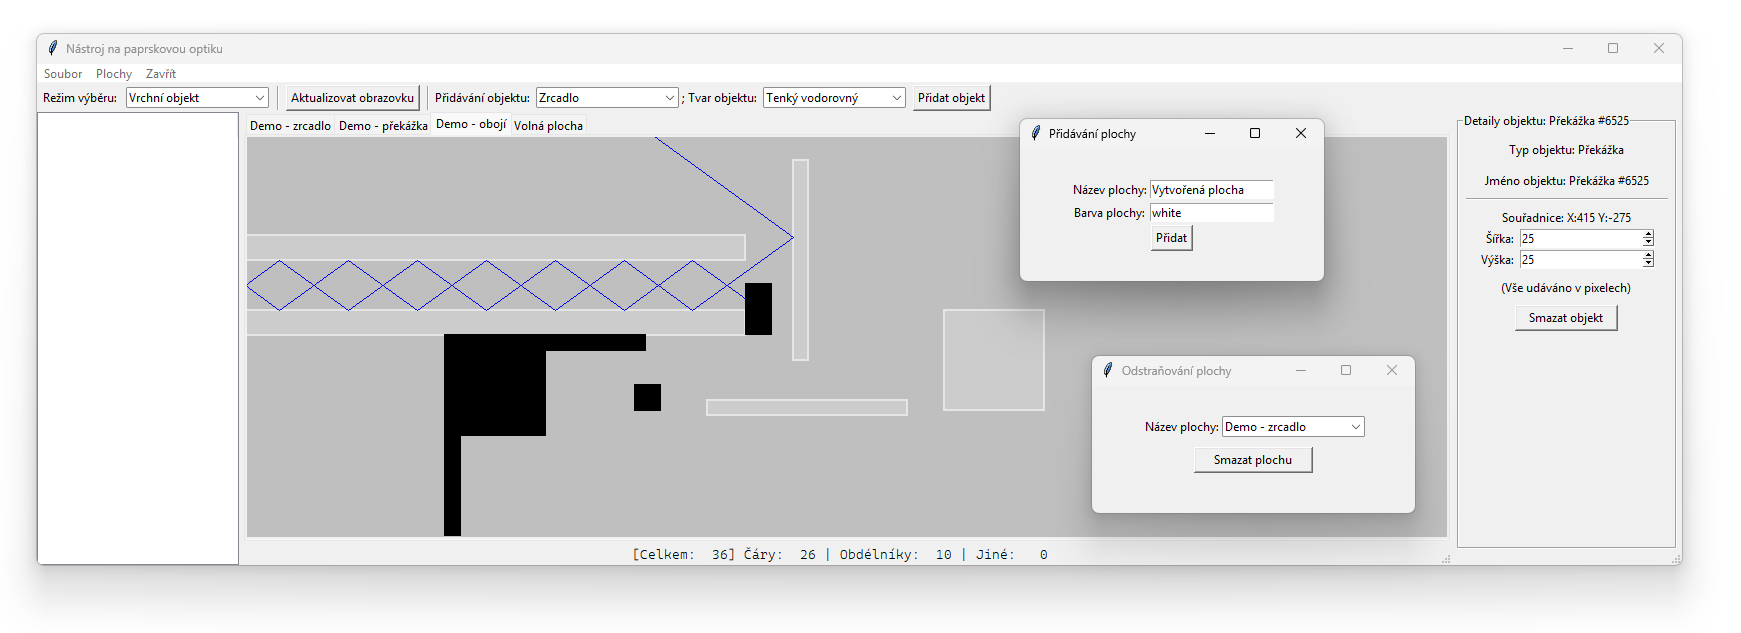
\includegraphics[width=1\linewidth]{Reference_GUI.png}
    \caption{Referenční snímek GUI včetně vyskakovacích oken}
    \label{fig:placeholder}
\end{figure}
\newpage \section{Použití}
\paragraph{Tlačítka v horní liště menu:}
\begin{itemize}
    \item Uložení/načtení souboru: Po otevření menu "Soubor"{} můžete uložit do souboru aktuálně vybranou plochu nebo načíst soubor tímto způsobem dříve uložený. Na příponě souboru nezáleží. Ukládá se název plochy, barva pozadí plochy, obsažené zdroje paprsku a obsažená zrcadla a překážky. Plocha z načteného souboru se objeví jako nová plocha v záložkách na vrchu hlavní části okna.
    \item Přidání a smazání plochy: Po otevření menu "Plochy"{} stiskněte patřičné tlačítko a tím se otevře okno, kde můžete vybrat detaily a akci provést. U přidávání plochy lze nastavit její jméno, které se zobrazí nad ní jako titulek její karty, a také barvu pozadí. Barvu pozadí vepisujte jako hex kód ve stylu \lstinline{"#00FF00"} nebo malými písmeny jako anglický název barvy. Slovní anglická pojmenování barev jsou podporována díky knihovně Tkinter, kterou můj program používá. U mazání plochy vyberete požadovanou plochu ve výběru ploch podle názvu. Vizte referenční snímek na předchozí stránce.
    \item Zavření: Použití tlačítka "Zavřít", křížku a zkratky \lstinline{Alt+F4} jsou ekvivalentní.
\end{itemize}
\paragraph{Hlavní plocha aplikace:}

\enlargethispage{1\baselineskip}
\begin{itemize}
    \item Výběr objektu: Na objekt klikněte nebo jím myší přetáhněte.
    \item Přemístění objektu: Na objektu podržte levé tlačítko myši a někam ho přesuňte, poté pusťte.
    \item Editování objektu: Po kliknutí na objekt se objeví detaily o něm v editovacím panelu vpravo. U zrcadel a překážek zde můžete měnit jejich výšku a šířku. To lze provádět vepsáním čísla, tlačítky napravo od vepisovacího pole, nebo šipkami nahoru a dolů na klávesnici (po kliknutí někam do vepisovacího pole).
    \item Přepnutí na jinou plochu: Použijte lištu nad pracovní plochou. Pak lze použít i šipky doleva a doprava na klávesnici.
    \item Změna velikosti okna: Rukojeti na jednodušší uchopení okna se nacházejí v pravém dolním rohu okna a také pod pravým dolním rohem prostředního panelu.
    \item Změna velikosti panelů: Rukojeti na pohyb hranicemi panelů najdete na předělech mezi panely.
\end{itemize}

\section{Režimy výběru myší}
\paragraph{} Vlastní implementace drag 'n drop systému je důležitá součást mého projektu. Implementoval jsem tři režimy, režim lze vybrat ve výběru vlevo nahoře v nástrojové liště. Defaultní je režim výběru jednoho objektu. Z objektů pod kurzorem vybere ten nejvíce v popředí. Režimy:
\begin{itemize}
    \item Vrchní objekt: Z objektů přímo pod kurzorem vybere ten nejvíce v popředí.
    \item Všechny pod kurzorem: Přetahování hýbe všemi objekty pod kurzorem, k editování je vybrán ten nejvíce v popředí.
    \item Zdroje světla: Vybere zdroje paprsků v těsné blízkosti kurzoru (není tedy potřeba trefit se úplně přesně, je zajištěno, že se kontroluje jistá oblast kolem kurzoru). Vybírají se zdroje paprsku, tedy je potřeba kliknout tam, kde paprsek začíná.
\end{itemize}

\section{Řešení problémů}
\paragraph{} Pokud se simulace na obrazovce chová jinak, než by měla, stačí obsah obrazovky aktualizovat a problém by měl hned být spraven. To lze udělat kliknutím na tlačítko "Aktualizovat"{} nahoře na liště nástrojů, nebo přetažením jakékoliv z překážek na obrazovce, protože to také způsobí celkovou aktualizaci obrazovky. Toto se může stát při přepnutí na novou obrazovku a tlačítko "Aktualizovat"{} toto řeší. Nejjednoduším řešením je ale pohnout jakýmkoliv prvkem na ploše, čímž se obsah plochy také aktualizuje a vykreslení se opět hned opraví.

% Závěr
\chapter{Závěr}
\paragraph{} GUI se mi podařilo, jsem s ním spokojený. V aktuálním stavu funguje, jak by mělo a je zajištěno, že do budoucna do něj lze přidávat všechno, co může být potřeba.
\paragraph{} Původně jsem zamýšlel, aby pracovní plochy byly scrollovatelné, ale to jsem v této verzi projektu nakonec neimplementoval. Zjistil jsem během práce, že by to bylo náročnější než jiné funkce, které pokládám za důležitější, zatímco přínos by nebyl tak vysoký.
\paragraph{} Simulační část je místo, kde můj projekt pokulhává. Simulace ve svém aktuálním stavu postrádá řadu funkcí. Rozhodl jsem se místo vytáření mnoha pokročilých funkcí vytvořit solidní základ, na kterém je možné pokročilejší simulaci vystavět.
\paragraph{} Systém základu simulace a kód pro kolize pochází ode mě za pomoci \href{https://paulbourke.net/geometry/pointlineplane/}{zdrojů o 2D analytické geometrii}. Toto bylo největší úskalí projektu a rozhodnutí tvořit vlastní systém simulace byla chyba, která stála tolik úsilí, které potom chybělo na vypracování částí projektu, které jsou více viditelné a na jejichž tvorbu jsem se při plánování těšil.
\paragraph{} Dále po maturitě bych tedy rád pokračoval v přidávání dalších a dalších funkcí tomuto projektu a jako první určitě chci vylepšit způsoby přidávání prvků na obrazovku, jakožto i možnosti editoru prvků. Kromě toho se chci ve větším klidu podívat na to, jak se počítají interakce s rozličnými optickými prvky a přidat Snellův zákon, který byl součástí mého původního plánu a který jsem musel kvůli nedostatku času na naprogramování systému na výpočty dalšího optického zákona prozatím opustit.
\enlargethispage{1\baselineskip}
\paragraph{} Během práce jsem se také naučil pracovat s verzovacím systémem Git, který v repertoáru správného programátora nesmí chybět a který odteď budu pro své projekty používat. V rámci maturitního projektu jsem tedy získal i tuto nepostradatelnou schopnost.
\paragraph{} Naučil jsem se i další, snad ještě víc důležitější věc, a tou je fakt, že rozvrhnout si projekt a posoudit, co vlastně zvládnu a co ne, je těžké. Při vymýšlení tématu jsem nepředvídal problémy, které pak při práci nastaly, a doplatil jsem na to.
\paragraph{} Cíl, který jsem si stanovil na začátku byl rozsáhlý a až příliš ambiciózní a v průběhu tvorby jsem musel udělat kompromisy, které znamenaly, že jsem prioritizoval funkční a stabilní základ jakožto i GUI a neimplementoval jsem pokročilejší funkce v simulační části, jako třeba systém materiálů a Snellův zákon. I přesto se práce na simulaci stala nejvíce problematickou částí celé mé práce, kupříkladu na tvorbě kódu pro kolizi přímky s úsečkou a následném řešení problémů s touto funkcí se moje práce zasekla na několik týdnů, což negativně ovlivnilo můj celkový dojem z realizace projektu.
\paragraph{} Nakonec se mi ale podařilo i tuto část doladit a provést přidání aspoň nejdůležitějších funkcí, které můj projekt potřeboval. Přestože v simulační části můj projekt postrádá hloubku, jsem s výsledkem svého snažení spokojený.
\end{document}